\def\currentRootFolder{chapter/energyDependentCrossSec}
\def\currentFigureFolder{\currentRootFolder/fig}
\newcommand{\sigmaInel}{\sigma_\mathrm{inel}}
\newcommand{\sigmaAvg}{\sigma_\mathrm{avg}}

\newcommand{\qUmin}{qU_\mathrm{min}}

\newcommand{\Ekin}{E_\mathrm{kin}}
\newcommand{\nSource}{n_\mathrm{S}}
\newacronym{standardmodel}{SM}{Standard Model of Particle Physics}
\newacronym{lep}{LEP}{Large Electron Positron Collider}
\newacronym{ssm}{SSM}{standard solar model}
\chapter{Energy-Dependence of the Cross Section for Inelastic Electron Scattering within the \glsentryshort{wgts}}
\label{sec:eDepScatCrossSec}
The probability of an electron to scatter when traveling through the \gls{wgts} can be characterized by the total scattering cross section $\sigma_\mathrm{tot}$. Two types of scatterings can be distinguished: elastic and inelastic scattering. The cross section for elastic scattering is by smaller than the one for inelastic scattering by one order of magnitude~\cite{Kleesiek2019}. This chapter focuses on inelastic scattering and neglects the other. Within this chapter, the cross section for electrons scattering inelastically off tritium molecules is just denoted as ``cross section'' and with the symbol $\sigma$. For ease of notation and reading, the adjective ``inelastic'' and an index such as ``inel'' is omitted where the context allows it unambiguously.

The cross section depends on the energy of the incident electrons: $\sigma \equiv \sigma(\Ekin)$. This dependence has been neglected in the formal modeling of a KATRIN measurement within the previous chapter~\ref{sec:intSpecModel}. This chapter investigates effects related to the incorporation of the energy-dependence. Section~\ref{sec:eDepScatCrossSecSources} lists cross section values from different sources and relates them to each other. Section~\ref{sec:eDepScatCrossSecModel} extends the mathematical formalism for a KATRIN measurement in order to incorporate the energy-dependence of the scattering cross section. Section~\ref{sec:eDepScatCrossSecNuMassInf} discusses the energy-dependence within the context of neutrino mass inference. In the end, section~\ref{sec:eDepScatCrossSecConclusion} concludes and offers an outlook.


\section{Cross Section for Electrons Scattering off Molecules of Hydrogen Isotopologues}
\label{sec:eDepScatCrossSecSources}
There exist several sources for cross-section formulae and values. This section gives an overview about the sources considered in this thesis and how they relate to each other. First, the cross section for electrons with an energy of \SI{18600}{eV} scattering off tritium was measured at the Troitsk experiment to be~\cite{Aseev2000}
\begin{equation}
	\sigma(\SI{18600}{eV}) = \SI{3.40\pm0.07e-22}{m^{-22}} \fullstop
\end{equation}
Also, the KATRIN Design Report lists a reference value~\cite{Angrik:2005ep}
\begin{equation}
	\label{eq:eDepScatCrossSecSourcesCrossSecTDR}
	\sigma_\mathrm{TDR} = \SI{3.456e-22}{m^{-2}} \fullstop
\end{equation}
Furthermore, there exist theoretical calculations of the cross section for electrons scattering of hydrogen molecules. In section~\ref{sec:eDepScatCrossSecSourcesTheory} the theoretical formulae are reviewed. How the different sources relate to each other and what approach is chosen within the scope of this thesis is explained in section~\ref{sec:eDepScatCrossSecSourcesChoice}.
\subsection{Theoretical Formulae}
\label{sec:eDepScatCrossSecSourcesTheory}
An expression for the inelastic cross section for electrons scattering off hydrogen molecules can be found in~\cite{Liu1973}. Two expressions are given, one for relativistic incident electrons and one for non-relativistic incident electrons. With regard to KATRIN the energies of $\upbeta$ electrons from tritium $\upbeta$ decay are relevant. The maximum relativistic $\beta$ factor of electrons from tritium $\upbeta$ decay is
\begin{align}
\beta(\Ekin, m) &= 
\sqrt{
	1-\frac{1}{
		(\frac{\Ekin}{m}+1)^2
	}
} \label{eq:eDepScatCrossSecSourcesCrossSecBetaFactor} \\
\Rightarrow\beta_\mathrm{max, T} &= 
\beta(\Eeff\approx\SI{18.6}{keV}, m_\elecIndex\approx\SI{511}{keV})\approx0.26 
\fullstop
\end{align}
Traveling at approximately a forth of the speed of light, the $\upbeta$ electrons are assumed to behave non-relativistic. Then, the given expression for the energy-dependent cross section is~\cite{Liu1973}
\begin{equation}
\label{eq:eDepScatCrossSecSourcesCrossSecLiu}
\sigma(E) =  
(4 \pi a_0^2) \cdot
\left(\frac{E}{R}\right)^{-1} \cdot
\left[
C_1 \cdot \ln{\left(\frac{E}{R}\right)} + C_2
\right]
\end{equation}
with the Bohr radius\footnote{Bohr radius $a_0=\SI[separate-uncertainty=false]{0.529 177 210 67(12)e-10}{m}$~\cite{ReviewOfParticlePhysics}} $a_0$, 
the Rydberg energy\footnote{Rydberg energy $R=\SI[separate-uncertainty=false]{13.605 693 009(84)}{eV}$~\cite{ReviewOfParticlePhysics}} $R$ and two constants $C_1$ and $C_2$. The later two depend on the hydrogen isotopologue. Different values a stated in different works for isotopic hydrogen
\begin{subequations}
\label{eq:eDepScatCrossSecSourcesCrossSecLiuConstants}
\begin{align}
C_1 &= 1.5487 &&\text{\cite{Liu1973}}
\label{eq:eDepScatCrossSecSourcesCrossSecLiuConstantsC1}\\[10pt]
C_2 &= 2.2212\pm0.0434 &&\text{\cite{Liu1973}}
\label{eq:eDepScatCrossSecSourcesCrossSecLiuConstantsC2Uncert}\\
C_2 &= 1.53 &&\text{\cite{Gerhart1975}} \\
C_2 &= 2.4036 &&\text{\cite{Liu1987}}
\label{eq:eDepScatCrossSecSourcesCrossSecLiuConstantsC2}
\fullstop
\end{align}
\end{subequations}
The latest of these references~\cite{Liu1987} acknowledges that the listed values for $C_2$ are not compatible. Within this work, the value from~\cite{Liu1987} is chosen as it is the most up-to-date of the listed ones. 

In equation~\eqref{eq:eDepScatCrossSecSourcesCrossSecLiu}, $E$ denotes\footnote{I would like to thank F. Glück for pointing this out.}
\begin{equation}
	\label{eq:eDepScatCrossSecSourcesCrossSecNonRelEnergy}
	E \equiv E(\Ekin) = \frac{1}{2} m_\elecIndex \beta^2(\Ekin, m_\elecIndex)
\end{equation}
with $\beta$ as in equation~\eqref{eq:eDepScatCrossSecSourcesCrossSecBetaFactor}. Figure~\ref{fig:eDepScatCrossSecSourcesValues} shows the theoretical cross-section formula along with the measured value by the Troitsk experiment and the value from the KATRIN Design Report.
\begin{figure}[t]
	\centering
	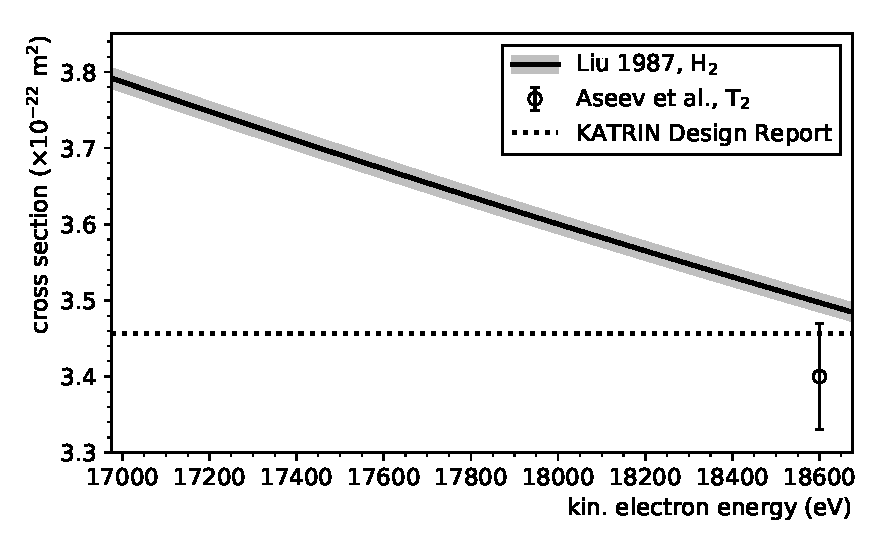
\includegraphics[width=\textwidth]{\currentFigureFolder/crossSecNoZoom.pdf}
	\xcaption{Inelastic cross section for non-relativistic incident electrons scattering off molecular hydrogen isotopologues}{Inelastic cross section for non-relativistic incident electrons scattering off molecular hydrogen isotopologues.}{Shown is the theoretical calculation according to equation~\eqref{eq:eDepScatCrossSecSourcesCrossSecLiu} with constants from equation~\eqref{eq:eDepScatCrossSecSourcesCrossSecLiuConstantsC1} and~\eqref{eq:eDepScatCrossSecSourcesCrossSecLiuConstantsC2} where the later is assumed to have an uncertainty according to equation~\eqref{eq:eDepScatCrossSecSourcesCrossSecLiuConstantsC2Uncert}. Also shown is the measurement by~\cite{Aseev2000} at the Troitsk experiment and the value stated in the KATRIN Design Report~\cite{Angrik:2005ep}. The shown energy interval is chosen according to the \gls{mtd} of the \gls{ft} measurement campaign.}
	\label{fig:eDepScatCrossSecSourcesValues}
\end{figure}

\subsection{Relation to Former Works}
\label{sec:eDepScatCrossSecSourcesChoice}
As can be seen in figure~\ref{fig:eDepScatCrossSecSourcesValues}, the cross section from the KATRIN Design Report does not match the theoretical calculations used in this thesis. However, the value stated in the KATRIN Design Report can be recovered from equation~\eqref{eq:eDepScatCrossSecSourcesCrossSecLiu}. If instead of the energy interpretation
of equation~\ref{eq:eDepScatCrossSecSourcesCrossSecNonRelEnergy}, one applies the interpretation
\begin{equation}
	\label{eq:eDepScatCrossSecSourcesCrossSecTDREngeryInterpretation}
	E \equiv \Ekin
	\fullstop
\end{equation}
The obtained cross section is $\sigma(\Ekin \approx \SI{18564.4}{eV}) = \SI{3.456e-22}{m^2}$ as stated in the KATRIN Design Report where the energy \SI{18564.4}{eV} is within the KATRIN design analysis interval (see section~\ref{sec:intSpecModelMTD}). This work applies the energy interpretation~\eqref{eq:eDepScatCrossSecSourcesCrossSecTDREngeryInterpretation} when comparability to former work is of importance. Otherwise, interpretation~\eqref{eq:eDepScatCrossSecSourcesCrossSecNonRelEnergy} is used\footnote{The cross sections obtained from the theoretical formula~\eqref{eq:eDepScatCrossSecSourcesCrossSecLiu} applying the energy interpretation via equation~\eqref{eq:eDepScatCrossSecSourcesCrossSecNonRelEnergy} are in better agreement with recently taken data at KATRIN according to preliminary analysis results by dedicated subgroups of the KATRIN collaboration at the time of writing this thesis.}. Corresponding indications are given. The quantitative difference of these two interpretations can be assessed by expanding the $\beta$ factor~\eqref{eq:eDepScatCrossSecSourcesCrossSecBetaFactor} in the ratio $\Ekin/m_\elecIndex \approx 18.575/511 \approx 0.036 \ll 1$
\begin{equation}
	\beta^2 \approx 
	2 \frac{\Ekin}{m_\elecIndex} - 
	3 \left(\frac{\Ekin}{m_\elecIndex}\right)^2
\end{equation}
The energy interpretation of equation~\eqref{eq:eDepScatCrossSecSourcesCrossSecNonRelEnergy} then becomes
\begin{equation}
	E(\Ekin) \approx 0.95 \Ekin
\end{equation}
which is a shift in energy and hence in the cross section of about \SI{5}{\percent} compared to the interpretation in~\eqref{eq:eDepScatCrossSecSourcesCrossSecTDREngeryInterpretation}. Exact calculations are given in the subsequent sections.

\section{An Energy-Dependent Scattering Model within the KATRIN Formalism}
\label{sec:eDepScatCrossSecModel}
The energy-dependence of the cross section enters into the calculation of the scattering probabilities~\eqref{eq:intSpecModelNonAveragedScatProbs}. In the derivation, that is given in the previous section~\ref{sec:intSpecModelResponseScattering}, the dependence on the starting energy $\Esource$ of electrons is neglected. Instead an average starting energy and hence, an average scattering cross section
\begin{equation}
	\label{eq:eDepScatCrossSecModelTRDCrossSec}
	\sigma(\SI{18564.37463}{eV})=\SI{3.456e-22}{m^2}
\end{equation}  (energy interpretation as per equation~\ref{eq:eDepScatCrossSecSourcesCrossSecTDREngeryInterpretation}) is assumed. Table~\ref{tab:eDepScatCrossSecModelScatProbs} lists the corresponding scattering probabilities averaged over all starting positions and pitch angles of electrons. Additionally, the results of a Monte-Carlo simulation by~\cite{Groh2015} and the values using the energy interpretation of equation~\eqref{eq:eDepScatCrossSecSourcesCrossSecNonRelEnergy} are given. How the energy-dependence of the scattering probabilities can be modeled is shown in section~\ref{sec:eDepScatCrossSecModelDescription}.  Subsequently, section~\ref{sec:eDepScatCrossSecModelDiscussion} discusses the presented model.

\begin{table}[t]
	\centering
	\xcaption{Probabilities for severalfold scattering of electrons in the \gls{wgts}}{Probabilities for severalfold scattering of electrons in the \gls{wgts}}{averaged over all starting positions and starting pitch angles. Both, the values from a Monte Carlo (MC) simulation and the values according to equation~\eqref{eq:intSpecModelAveragedScatProbs} are given. The  cross section was evaluated at an energy of $E=\SI{18564.37463}{eV}$ 
	for the two energy interpretations described by equation~\eqref{eq:eDepScatCrossSecSourcesCrossSecTDREngeryInterpretation} and~\eqref{eq:eDepScatCrossSecSourcesCrossSecNonRelEnergy}. Further input parameters to the calculations are a constant gas column density $\rho d = \SI{5e17}{cm^{-2}}$, 
	a \gls{wgts} length of $d=\SI{10.0820}{m}$
	and a maximum acceptance angle of $\thetaMax=\SI{50.7685}{\degree}$.}
	\begin{tabular}{lllr}
		\toprule
		\makecell[tl]{cross section (\SI{e-22}{m^{-2}}) $\rightarrow$} &
		3.456 &
		3.456 &
		3.673 \\
		\hline
		\makecell[tl]{source $\rightarrow$} & 
		\makecell[tl]{MC particle tracking\\ \cite{Groh2015}} & 
		\makecell[tl]{eq. \eqref{eq:intSpecModelAveragedScatProbs} \\ \cite{Groh2015, Kleesiek2014}} &
		\makecell[tr]{eq. \eqref{eq:intSpecModelAveragedScatProbs}}
		\\
		\hline
		\makecell[cl]{scattering count $\downarrow$} & 
		& 
	    & \\
		\hline
		\makecell{0} & $0.415 \pm 0.002$ & 0.41334 & 0.39564 \\
		\makecell{1} & $0.292 \pm 0.002$ & 0.29266 & 0.28967 \\
		\makecell{2} & $0.166 \pm 0.001$ & 0.16733 & 0.17298 \\
		\makecell{3} & $0.079 \pm 0.001$ & 0.07913 & 0.08590 \\
		\makecell{4} & $0.031 \pm 0.001$ & 0.03178 & 0.03634 \\
		\bottomrule
	\end{tabular}
	\label{tab:eDepScatCrossSecModelScatProbs}
\end{table}


\subsection{Model Description}
\label{sec:eDepScatCrossSecModelDescription}
\begin{figure}[th]
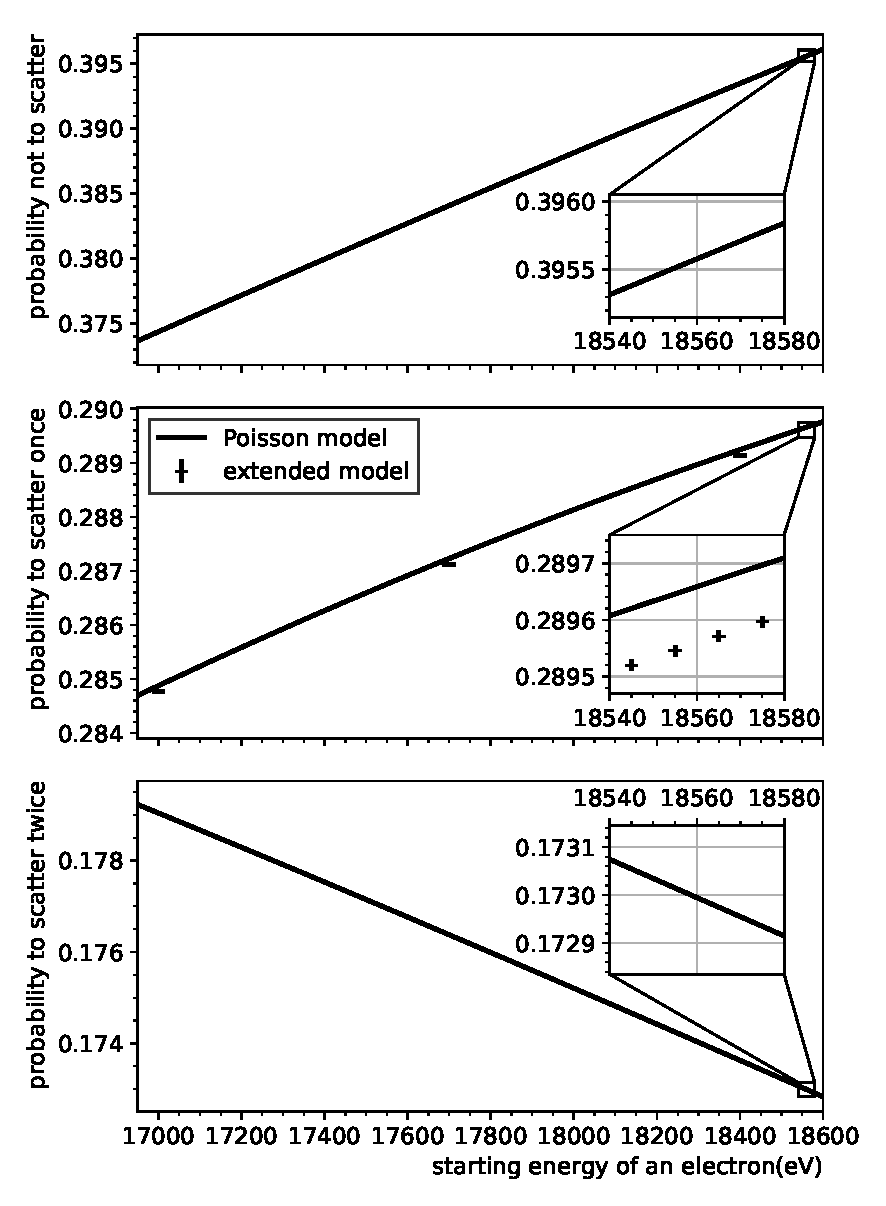
\includegraphics[width=\textwidth]{\currentFigureFolder/scatProbs012.pdf}
        \xcaption{Energy-dependent probabilities for electron scattering within the \gls{wgts}}{Energy-dependent probabilities for electron scattering within the \gls{wgts}.}{From top to bottom the probability for no, one-fold and two-fold scattering are shown averaged over all starting positions and starting pitch angles of electrons within the \gls{wgts}. The lines show the Poisson model and the markers the extended model (see main text for a description of the models). The extended model is only shown for one-fold scattering because for no scattering, it equals the Poisson model and for two-fold scattering it was not calculated (see appendix~\ref{sec:appendixEDepScatCrossSecExtendedModel} for an explanation). The numerical evaluation of the extended model is subject to an uncertainty of $\sim10^{-5}$ (see appendix~\ref{sec:appendixEDepScatCrossSecExtendedModelNumEval}), that is depicted as uncertainty bars. The shown energy range matches the measurement range of the \glsentryfull{ft} measurement campaign and the inset shows an energy span around the endpoint of the tritium $\upbeta$ spectrum.}
        \label{fig:eDepScatCrossSecModel}
\end{figure}
Within this section, two models are presented in order to incorporate the energy-dependence of the scattering cross section into the mathematical formalism of a KATRIN measurement.

\paragraph{Poisson Model}
An expression for the probability of $l$-fold scattering of electrons within the \gls{wgts} is derived in the previous section~\ref{sec:intSpecModelResponseScattering}. The given model is independent of the energy of the electrons. Instead of using a constant cross section, the energy-dependence can be respected. The corresponding formulae from section~\ref{sec:intSpecModelResponseScattering} are repeated below, with the energy-dependence made explicit
\begin{subequations}
\label{eq:eDepScatCrossSecModelPoisson}
\begin{align}
    \mu(\Esource,\zSource,\thetaSource) =&
    \frac{\sigma(\Esource)}{\cos\thetaSource}
    \int_{\zSource}^{d/2} \rho(z)\d z \label{eq:energydepScatProbsPoissonExpectedScatCount} \\
    P_l(\Esource,\zSource,\thetaSource) =&
    \mathrm{Poisson}(\mu(\Esource,\zSource,\thetaSource),l) \label{eq:eDepScatCrossSecModelPoissonNonAveragedScatProbs} \\
    \bar{P}_l(\Esource) =&
    \frac{1}{d \cdot (1-\cos(\thetaMax))} 
      \int_{-d/2}^{d/2}  
          \int_{0}^{\theta_{max}} 
            \sin(\thetaSource)
            \mathrm{Poisson}(\mu(\Esource,\zSource,\thetaSource),l)
          \d\thetaSource
      \d\zSource
      \label{eq:eDepScatCrossSecModelPoissonAveragedScatProbs}
    \fullstop
\end{align}
\end{subequations}
As a reminder, $\bar{P}_l(\Esource)$ in the final equation \eqref{eq:eDepScatCrossSecModelPoissonAveragedScatProbs} denotes the probability of $l$-fold scattering for a $\upbeta$ electron with a starting energy $\Esource$ averaged over all starting positions and pitch angles. In the following, this model is denoted ``Poisson model''. It is expected to be accurate for the probability of no scattering $\bar{P}_0(\Esource)$. But, depending on the required accuracy, for one or more scatterings the Poisson model does not necessarily hold as explained in the following paragraph.

\paragraph{Extended Model}
A scattering electron loses energy. The scattering cross section increases with decreasing energies and the electron becomes more likely to scatter again. In other words, the probabilities of individual scattering processes are no longer independent when respecting the dependence on the electron energy. This violates one of the preconditions to model the scattering probabilities via a Poisson distribution. Another model is suggested that partly accounts for this fact (inspired by a model in~\cite{Groh2015} that incorporates changes of the electron pitch angle due to scattering). It assumes a fixed energy loss per scattering. A descriptive derivation is given in appendix~\ref{sec:appendixEDepScatCrossSecExtendedModel}. In this section it is labeled by
\begin{equation}
	\label{eq:eDepScatCrossSecModelExtended}
	\bar{P}^{\star}_l(\Esource)
\end{equation}
and it denotes the probability of $l$-fold scattering for a $\upbeta$ electron with a starting energy $\Esource$ averaged over all starting positions and pitch angles assuming a fixed energy loss $\epsilon$ per scattering. In the following, this model is denoted the ``extended model''. The value $\epsilon=\SI{12.6}{eV}$ was chosen as it is the most probable energy loss for electrons traveling through tritium gas (see figure~\ref{fig:intSpecModelAseevEloss}). A more accurate description would incorporate the full energy loss function. This may be the subject of a future study. 

The extended model was evaluated numerically as it includes one limit and two integrals (see appendix~\ref{sec:appendixEDepScatCrossSecExtendedModelFormalism}). The numerical accuracy had to be good enough to decided whether it differs significantly from the Poisson model or not. At the same time, a balance between the numerical accuracy and the evaluation run time had to be found. The probability for one-fold scattering could be calculated with a numerical accuracy on the $10^{-5}$ level (see appendix~\ref{sec:appendixEDepScatCrossSecExtendedModelNumEval} on how this value is derived and how it can be interpreted). However, the evaluation of the extended model for more than one scattering has not yet been done and may be the subject of a future study.

\subsection{Model Discussion}
\label{sec:eDepScatCrossSecModelDiscussion}
Figure~\ref{fig:eDepScatCrossSecModel} shows the Poisson model along with the suggested extended model. The results are discussed in the following paragraphs.

\paragraph{Model compatibility}
Table \ref{tab:eDepScatCrossSecModelScatProbs} lists the scattering probabilities for an energy-independent Poisson model (see section~\ref{sec:intSpecModelResponseScattering}) and a reference cross section $\sigma(\Ekin\approx\SI{18564.4}{eV})\approx\SI{3.673e-22}{m}$. The energy-dependent Poisson model recovers the energy-independent model exactly at the corresponding energy as expected. For the probability of one-fold scattering the difference between the Poisson and the extended model is below $10^{-4}$. How this difference propagates to neutrino mass inference was not further investigated in the scope of this thesis, but may be the subject of a future study. The \gls{ssc} software framework, used by many former works (e.\,g.~\cite{Groh2015,Kleesiek2014,SeitzM2019} evaluates the integrals within the scattering probabilities numerically with an accuracy of $10^{-5}$, which may serve as an indicator on to what extend the difference is of importance.

\paragraph{The Poisson Model as Probability Density}
In the following, it is shown that the energy-dependent Poisson model $\bar{P}_l(\Esource)$ (see equation~\ref{eq:eDepScatCrossSecModelPoisson}) resembles a probability density in $l$ independent of a constant starting energy~$\Esource$ of electrons because this can be used to explain further model properties. Accordingly, the two properties that have to be verified are
\begin{align}
	\forall \Esource > 0: \quad
	&\bar{P}_l(\Esource) > 0 \\
	&\sum_{l}^{\infty} \bar{P}_l(\Esource) = 1
	\fullstop
\end{align}
The fist condition holds because all quantities in the calculation of $\bar{P}_l(\Esource)$ are positive. For the second condition, one can use that the Poisson distribution is a probability density that sums to one
\begin{align*}
	\sum_{l}^{\infty} \bar{P}_l(\Esource) &=
	\frac{1}{d \cdot (1-\cos(\thetaMax))} 
	\int_{-d/2}^{d/2}  
	\int_{0}^{\theta_{max}} 
	\sin(\thetaSource)
		\sum_{l}^{\infty}
		\mathrm{Poisson}(\mu(\Esource,\zSource,\thetaSource),l)
	\d\thetaSource
	\d\zSource \\  &=
	\frac{1}{d \cdot (1-\cos(\thetaMax))} 
	\int_{-d/2}^{d/2}  
	\int_{0}^{\theta_{max}} 
	\sin(\thetaSource)
		\cdot 1
	\d\thetaSource
	\d\zSource \\ &= 1
	\fullstop
\end{align*}
This verifies that the Poisson model is a probability density in the amount of scatterings $l$.

\paragraph{Trend of energy-dependence}
As depcited in figure~\ref{fig:eDepScatCrossSecModel}, for an increasing starting energy of electrons within the \gls{wgts} the probability for no and one-fold scattering also increases, while the probability for two-fold scattering decreases. This paragraph aims at giving an intuitive argument for this change of sign in the derivative $\d \bar{P}_l(\Esource) / \d \Esource$ in the transition from $l=1$ to $l=2$. First, the expected scattering count for an energy within the depicted range $\Esource \in [\SI{17}{keV}, \SI{18.6}{keV}]$ of starting energies can be calculated numerically (the sum converges because $\bar{P}_l(\Esource)$ is a probability density as shown in the previous paragraph):
\begin{align}
	\bar{l}(\SI{17.0}{keV}) &= 
	\sum_{l}^{\infty} \bar{P}_l(\SI{17.0}{keV}) \cdot l \approx 1.23 \\	
	\bar{l}(\SI{18.6}{keV}) &= 
	\sum_{l}^{\infty} \bar{P}_l(\SI{18.6}{keV}) \cdot l \approx 1.14
	\fullstop
\end{align} 
In other words, electrons with a starting energy between \SI{17}{keV} and \SI{18.6}{keV} are expected to scatter between 1 and 2 times on their way through the \gls{wgts} (averaged over all starting positions and pitch angles). Then, the illustrative line of argument is the following: 
\begin{align*}
	&\text{ the starting energy $\Esource$ increases} \\ \Rightarrow
	&\text{ the scattering cross section decreases (see figure~\ref{fig:eDepScatCrossSecSourcesValues})} \\ \Rightarrow
	&\text{ scattering becomes less likely} \\ \Rightarrow
	&\text{ $\bar{l}$ decreases and moves closer to 1 and away from 2} \\ \Rightarrow
	&\text{ the probability for no and one-fold scattering increases,} \\
	&\text{ while the probability for more than one scattering decreases}
	\fullstop
\end{align*} 
This is in accordance with the trend of the energy-dependence depicted in figure~\ref{fig:eDepScatCrossSecModel}.
\FloatBarrier

\paragraph{Implementation and Performance}
Within the scope of this thesis, the energy-dependent Poisson model of equation~\eqref{eq:eDepScatCrossSecModelPoisson} was implemented into the \gls{ssc} software framework. The extended model of equation~\eqref{eq:eDepScatCrossSecModelExtended} was not further investigated in this work. The energy-dependence of the scattering cross section may not be negligible in neutrino mass inference as is explained in the subsequent section~\ref{sec:eDepScatCrossSecNuMassInf}. For that reason, the impact on the fitting run time by using an energy-dependent cross section was probed. Depending on the \gls{mtd}, a fit might become slower by a factor of 40 to 120. This is due to the fact, that, when integrating over the energy loss in the response function in equation~\eqref{eq:intSpecModelResponse}, the scattering probabilities have to be recomputed in every step of the numerical integration. It might be beneficial to investigate whether the evaluation can be speed up in the future.


\section{Effect on the Inferred Neutrino Mass}
\label{sec:eDepScatCrossSecNuMassInf}
\begin{figure}[t]
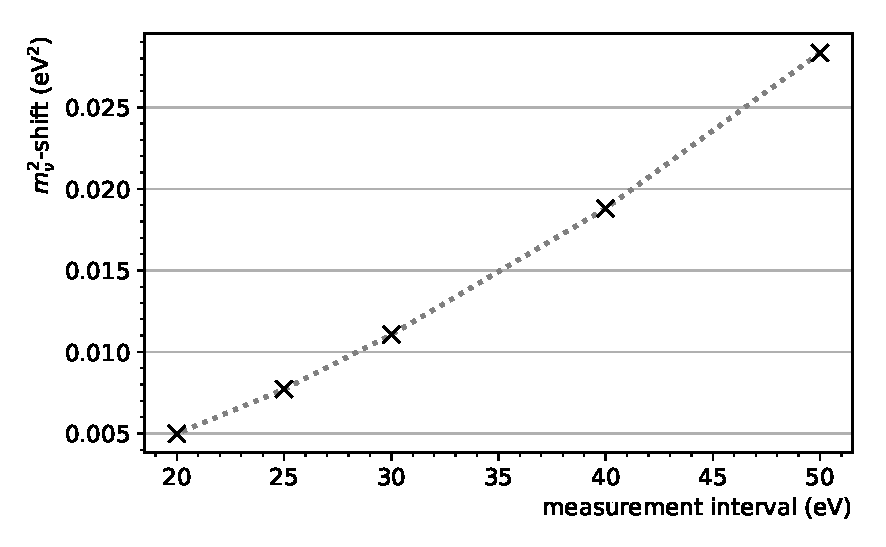
\includegraphics[width=\textwidth]{\currentFigureFolder/nuMassShiftForEDepCrossSec.pdf}
        \xcaption{Shift of an inferred squared neutrino mass induced by a neglected energy-dependence of the inelastic scattering cross section}{Shift of an inferred squared neutrino mass induced by a neglected energy-dependence of the inelastic scattering cross section.}{The neutrino mass was inferred from data that was simulated using an energy-dependent inelastic scattering cross section as per equation~\ref{eq:eDepScatCrossSecSourcesCrossSecLiu} with the energy interpretation of~\ref{eq:eDepScatCrossSecSourcesCrossSecTDREngeryInterpretation} using a fit model that assumes a constant cross section of $\sigma_\mathrm{TDR}=\SI{3.456e-22}{m^{-22}}$. The procedure was repeated for the five different \gls{mtd}s given in the KATRIN design report.}
        \label{fig:eDepScatCrossSecNuMassInfShifts}
\end{figure}
It was investigated how much the squared neutrino mass that is inferred from a KATRIN measurement would be shifted if the energy-dependence of the scattering cross section is neglected in the corresponding fitting procedure. The comparability to former results is of importance within this section. For that reason, the energy interpretation of equation~\ref{eq:eDepScatCrossSecSourcesCrossSecTDREngeryInterpretation} is used, which yields a cross section of $\sigma_\mathrm{TDR}=\SI{3.456e-22}{m^{-2}}$~\cite{Angrik:2005ep} within the KATRIN design analysis interval.

There are several previous works that studied similar effects~\cite{Antoni2015,Groh2015,SeitzM2019,Kuckert2016,Kuckert2018}. Before the results of this thesis are presented, the results from~\cite{Groh2015} are reviewed representatively for the mentioned works. The review is presented, because the former results might intuitively contradict the results obtained in this thesis. Then, the results of this thesis are listed and an argument is given, why both sets of results are probably in accordance.

In~\cite{Groh2015}, it was investigated how much a constant offset of the cross section would shift the inferred squared neutrino mass if the offset were neglected in the analysis. A rule of thumb for the shift in dependence on the relative offset of the cross section $\Delta\sigma/\sigma_\mathrm{TDR}$ is given~\cite{Groh2015}
\begin{equation}
	\label{eq:eDepScatCrossSecNuMassInfShiftRuleOfThumb}
	\frac{\Delta\nuMass^2(\Delta\sigma)}{\SI{e-3}{eV^2}} =
	-0.45
	-1204\cdot
	\frac{
		\Delta\sigma
	}{
		\sigma_\mathrm{TDR}
	}
	\qquad \text{ with } \quad 
	\sigma_\mathrm{TDR} = \SI{3.456e-22}{m^{-2}}
	\fullstop
\end{equation}
Due to the energy dependence, in the KATRIN design analysis interval of \SI{30}{eV}, the relative offset of the cross section is
\begin{equation}
	\label{eq:eDepScatCrossSecNuMassInfRelativeCrossSecOffset}
	\left|
	\frac{
		\Delta\sigma
	}{
		\sigma_\mathrm{TDR}
	}
	\right| < \SI{0.1}{\percent}
	\fullstop
\end{equation}
Thus, the rule of thumb~\ref{eq:eDepScatCrossSecNuMassInfShiftRuleOfThumb} yields
\begin{equation}
	\label{eq:eDepScatCrossSecNuMassInfShiftEstimate}
	\left|
		\Delta\nuMass^2(\Delta\sigma)
	\right| < \SI{2e-3}{eV^2} 
	\fullstop
\end{equation}
In the following, the results of this thesis are presented and related to the obtained estimate~\eqref{eq:eDepScatCrossSecNuMassInfShiftEstimate}.
In the scope of this thesis, an energy-dependent offset of the cross section was investigated (in contrast to a constant one in~\cite{Groh2015}). A KATRIN neutrino mass measurement for a neutrino mass of \SI{0}{eV} was simulated using an energy-dependent cross section\footnote{In all studies presented in this chapter, the simulated electron detector counts were substituted by their expectation values as opposed to fluctuated according to Poissonian statistics. In other words, no ensemble testing was done. For more details on such an Asimov data, see section~\ref{sec:katrinElossStatisticsAsimov}.}. A model that uses a constant cross section was fitted to the simulated spectrum. This procedure was repeated for the five different \gls{mtd}s given in the KATRIN Design Report. Figure~\ref{fig:eDepScatCrossSecNuMassInfShifts} shows the results. For the~\SI{30}{eV} measurement interval, the difference from \SI{0}{eV} respectively the shift of the squared neutrino mass is
\begin{equation}
	\Delta\nuMass^2 = \SI{1.09e-2}{eV^2}
	\fullstop
\end{equation}
This shift is larger than the one listed above under equation~\eqref{eq:eDepScatCrossSecNuMassInfShiftEstimate}. This might be contra intuitive, but can be argued. The reason may be, that the fit parameter for the signal amplitude $\sigAmp$ in a nominal KATRIN fit (see section~\ref{sec:statMethodsStandardFit}) can compensate for a constant offset of the cross section. However, it may not compensate for an energy-dependent one. In order to verify this statement, two arguments are presented below.
First, the study from~\cite{Groh2015} was reproduced with a free fit parameter for the signal amplitude $\sigAmp$. The reproduced study was in accordance with the values in~\cite{Groh2015}. Then, $\sigAmp=1$ was fixed. The results are shown in figure~\ref{fig:eDepScatCrossSecNuMassInfShiftsForConstCrossSec}. A relative cross section offset of $
\left|
	\Delta\sigma/\sigma_\mathrm{TDR}
\right| \approx \SI{0.1}{\percent}
$ (see equation~\ref{eq:eDepScatCrossSecNuMassInfRelativeCrossSecOffset}) yields a shift of the squared neutrino mass, that is larger by almost an order of magnitude with a fixed $\sigAmp$ as opposed to leaving $\sigAmp$ as a free parameter. The shifts are then compatible with the shifts of the study presented in this chapter.

The second plausibility argument is the following: Figure~\ref{fig:eDepScatCrossSecNuMassInfShiftsForConstCrossSec} shows the simulated integral rate for different cross section models normalized to the integral rate obtained by using the constant cross section $\sigma_\mathrm{TDR}$ from the KATRIN Design Report. The integral rates that are based on a model with a constant (as in energy-independent) cross section differ from each other by almost a constant factor (variations $<2\times10^{-4}$ level). This implies, when one of these models is used in a simulation of a KATRIN measurement and another model is used in a corresponding fit for neutrino mass inference, their difference can be compensated by the fit parameter for the signal amplitude $\sigAmp$. However, the model that uses an energy-dependent cross section, does not differ from the one with the constant cross $\sigma_\mathrm{TDR}$ section by a constant factor. The difference varies over the energy range. Such a difference can not be compensated by the fit parameter for the signal amplitude $\sigAmp$.

The two presented arguments show that the results presented in this chapter and the ones in~\cite{Groh2015} do not necessarily contradict each other.

\begin{figure}[t]
	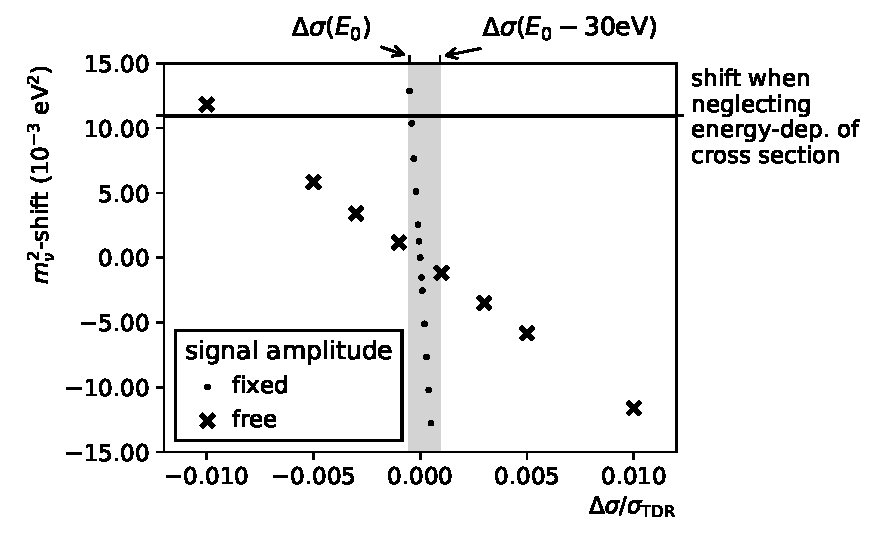
\includegraphics[width=\textwidth]{\currentFigureFolder/nuMassShiftForConstCrossSec.pdf}
	\xcaption{Shift of an inferred squared neutrino mass induced by a neglected constant offset of the inelastic scattering cross section}{Shift of an inferred squared neutrino mass induced by a neglected constant offset of the inelastic scattering cross section.}{The neutrino mass was inferred from data that was simulated using an inelastic scattering cross section of $\sigma_\mathrm{TDR}=\SI{3.456e-22}{m^{-22}}$. The x-axis shows the relative offset of the inelastic scattering cross section assumed in the inference process. In an energy-dependent scenario, a cross section corresponds an energy of incident electrons as per equation~\eqref{eq:eDepScatCrossSecSourcesCrossSecLiu}. The cross section range, that corresponds the design KATRIN analysis interval of \SI{30}{eV} is depicted as a gray band. The analysis was done twice: once with a free parameter for the signal amplitude, which reproduced the results given in~\cite{Groh2015}~(figure 6.31 on page 221); the second analysis had this parameter fixed. The shifts obtained with a fixed signal amplitude are compatible with the one obtained by neglecting the energy-dependence of the cross section within the \SI{30}{eV} measurement interval.}
	\label{fig:eDepScatCrossSecNuMassInfShiftsForConstCrossSec}
\end{figure}


\begin{figure}[t]
	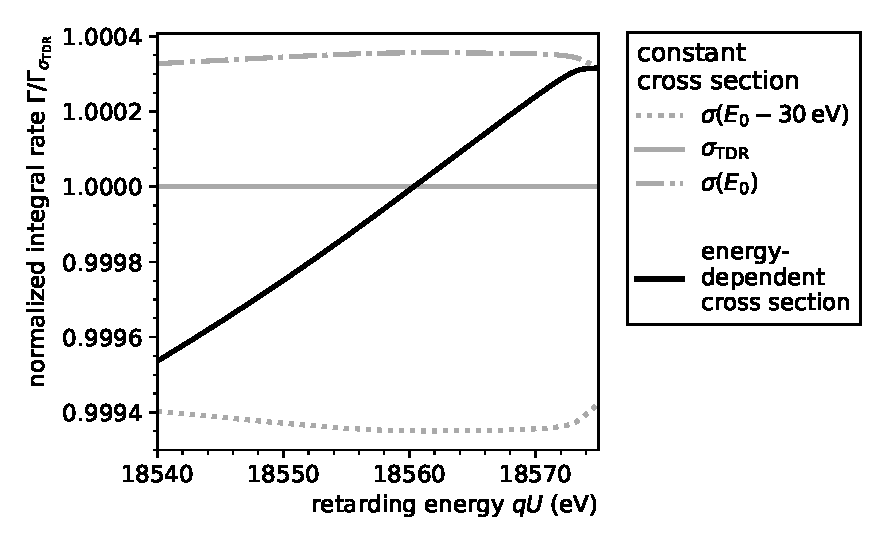
\includegraphics[width=\textwidth]{\currentFigureFolder/normedIntegralRate.pdf}
	\xcaption{Simulated integral $\boldsymbol{\upbeta}$-electron rate using different models of the cross section for inelastic electron scattering}{Simulated integral $\boldsymbol{\upbeta}$-electron rate using different models of the cross section for inelastic electron scattering.}{The x-axis shows the energy range of the design KATRIN analysis interval. The lines show the integral rate of $\upbeta$ electrons for different models for the inelastic scattering cross section normalized to the model, that uses the constant cross section $\sigma_\mathrm{TDR}=\SI{3.456e-22}{m^{-22}}$. The gray lines use a model with a constant cross section. The cross section values can be identified with electron energies as per equation~\eqref{eq:eDepScatCrossSecSourcesCrossSecLiu} and the energy interpretation of equation~\eqref{eq:eDepScatCrossSecSourcesCrossSecTDREngeryInterpretation} with $\sigma(E_0-\SI{30}{eV}=\SI{18545}{eV})=\SI{3.459e-22}{m^{-22}}$ and $\sigma(E_0=\SI{18575}{eV})=\SI{3.454e-22}{m^{-22}}$. The black line shows the simulated integral rate for an energy-dependent cross section. This graph is meant to emphasize that the integral rates for models using a constant cross section differ by an almost constant factor, whereas the rate using an energy-dependent cross section differs by a varying factor.}
	\label{fig:eDepScatCrossSecNuMassInfShiftsForConstCrossSec}
\end{figure}
\FloatBarrier
\section{Conclusion and Outlook}
\label{sec:eDepScatCrossSecConclusion}
The cross section for inelastic scattering off tritium molecules within the \gls{wgts} depends on the energy of the incident electrons. Two models were developed that can integrate this dependence into a mathematical description of a KATRIN neutrino mass measurement. Strong indications were found, that the energy-dependence of the scattering cross-section should not be neglected in neutrino mass inference as it could lead to a bias and shift the squared neutrino mass by $\Delta\nuMass^2 = \SI{1.09e-2}{eV^2}$ in a KATRIN design measurement interval of $\SI{30}{eV}$.

The model building was based on well argued considerations. Nonetheless, an independent cross-check is recommended. A future study might perform a Monte-Carlo simulation in order to verify the suggested models presented in this thesis. Furthermore, for the results in this thesis an approximation was made by modeling the probability for several-fold scattering via a Poisson distribution. It was shown, that this introduces an error of approximately $10^{-4}$ for the probability of one-fold scattering. Whether this effect is significant needs further investigation.

It was also shown, that including the energy-dependence in neutrino mass inference increases the run time of the fitting procedure. Future work might consider techniques beyond the scope of this thesis in order to speed up the calculation process.